\section{Procedimiento} 

Primeramente crearemos una base de datos llamada BDTEST.Abrir el SQL Server Data Tools y dirigirnos a la pestaña de Business Intelligence -> Analysis Services. Como se creará un Modelo Multidimensional desde 0 , seleccionaremos la primera opción. En la casilla de Name le colocamos un nombre al proyecto y a la solución:
	\begin{center}
	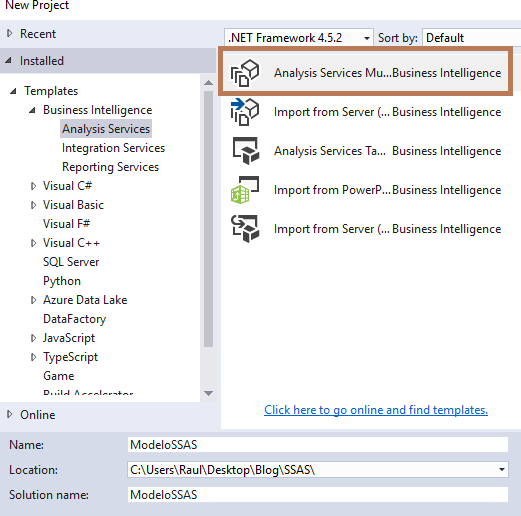
\includegraphics[width=0.5\columnwidth]{images/task1/1}
	\end{center}	

\section{Ejercicio 01 Creación de un proyecto de Analisys Services}

Crear un nuevo Proyecto en Visual Studio 2017.  Hacer clic en Business Intelligence
Seleccione el tipo de Proyecto multidimensional y de minería de datos de Analysis Services
	\begin{center}
	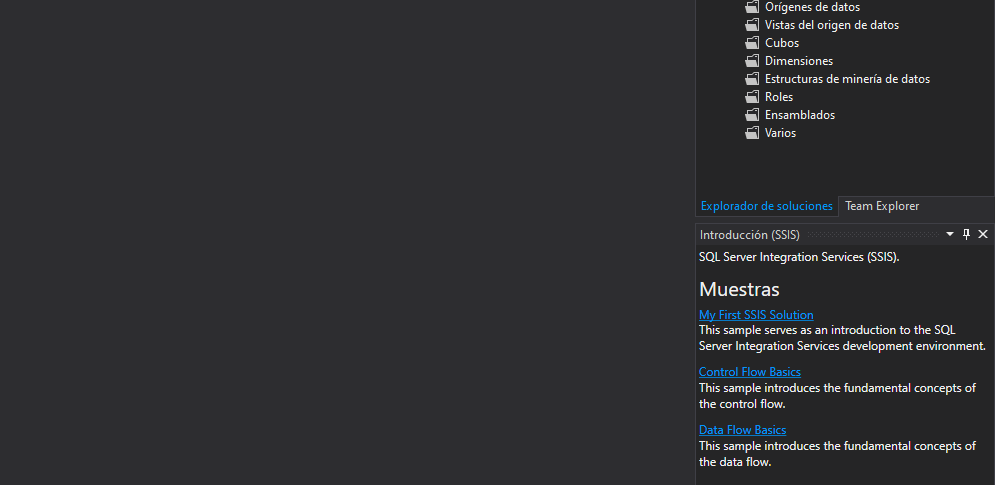
\includegraphics[width=0.5\columnwidth]{images/task1/2}
	\end{center}	

